\begin{figure}[h!]
    \begin{center}
        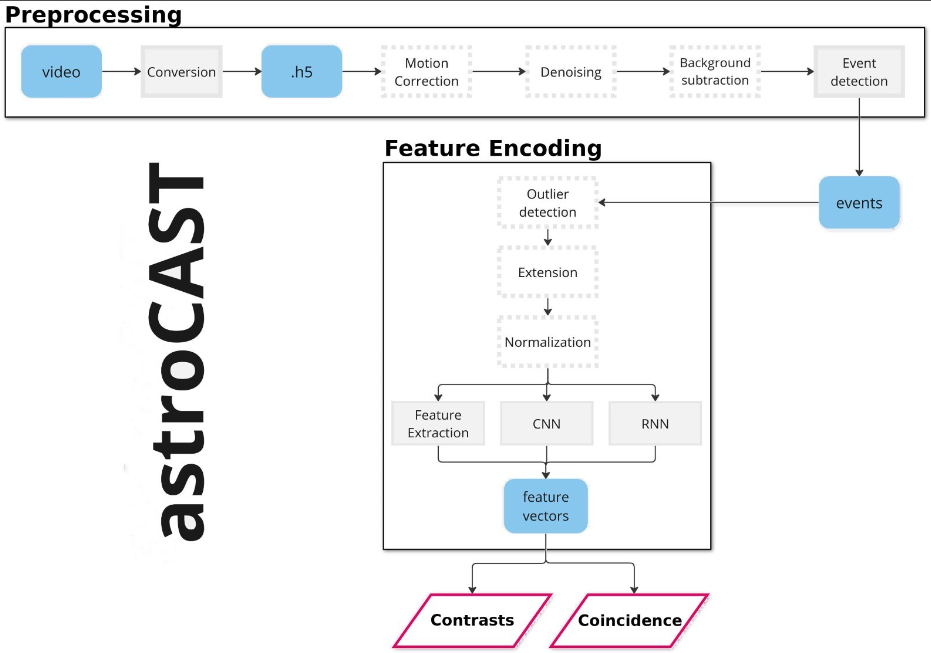
\includegraphics[width=\linewidth]{figures/1.png}
    \end{center}
    \caption{AstroCAST Pipeline Overview: First box shows how the input video is converted and processed to detect
    events. Second box shows how the detected events undergo feature extraction utilizing different approaches to
    generate feature vectors. Last steps shows how feature vectors can be analyzed to identify patterns and
    correlations. Optional steps in the pipeline are indicated by dotted boxes, and outputs at each stage are shown
    in blue. Exemplary types of experiments explained in this protocol are highlighted in red.

    }\label{fig:1}
\end{figure}

\begin{figure}[h!]
    \begin{center}
        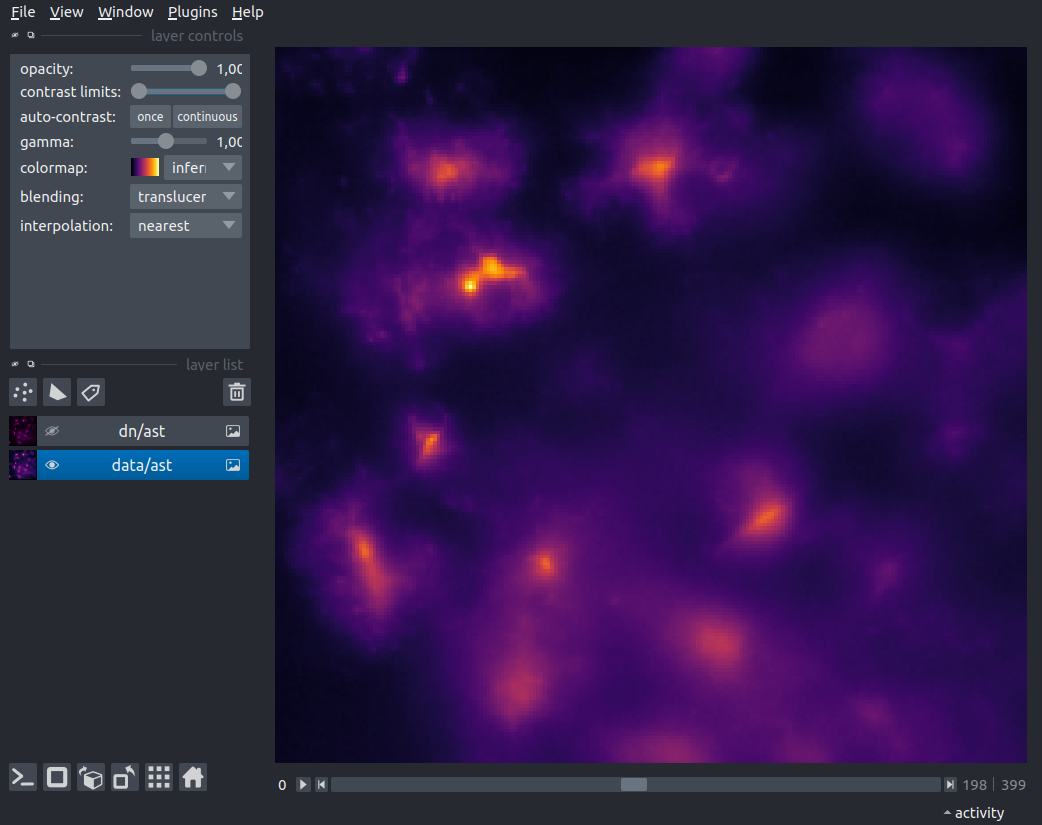
\includegraphics[width=\linewidth]{figures/2.png}
    \end{center}
    \caption{Screenshot of the \ac{GUI} displaying the converted video file of astrocytic calcium fluorescence (\ref{
        Tbl1}). The video has been downsampled and captured at a 20X magnification, focusing on the \ac{preBötC}
    region.}\label{fig:2}
\end{figure}

